\section{Konzeptentwurf der Cloud Infrastruktur}
\label{sec:cloud-infra}
In diesem Kapitel wird auf die verwendete Infrastruktur Architektur eingegangen. %Dabei sollen die zuvor aufgestellten Anforderungen an die Infrastruktur erfüllt werden. 
Dabei soll die Infrastruktur den Betrieb einer Cloud-nativen Anwendung ermöglichen. Die nachfolgende Abbildung gibt einen Überblick wie die einzelnen Komponenten miteinander kommunizieren und voneinander abhängen. Drüber hinaus werden einige Gründe für die Auswahl der Services aufgezeigt.

Im vorangehenden Kapitel \ref{sec:konzeptentwurf} wurde bereits die Wahl von \ac{AWS} getroffen und begründet. Bei den genutzten Services handelt es sich entsprechend um \ac{AWS} Services.

\begin{figure}[H]
    \centering
    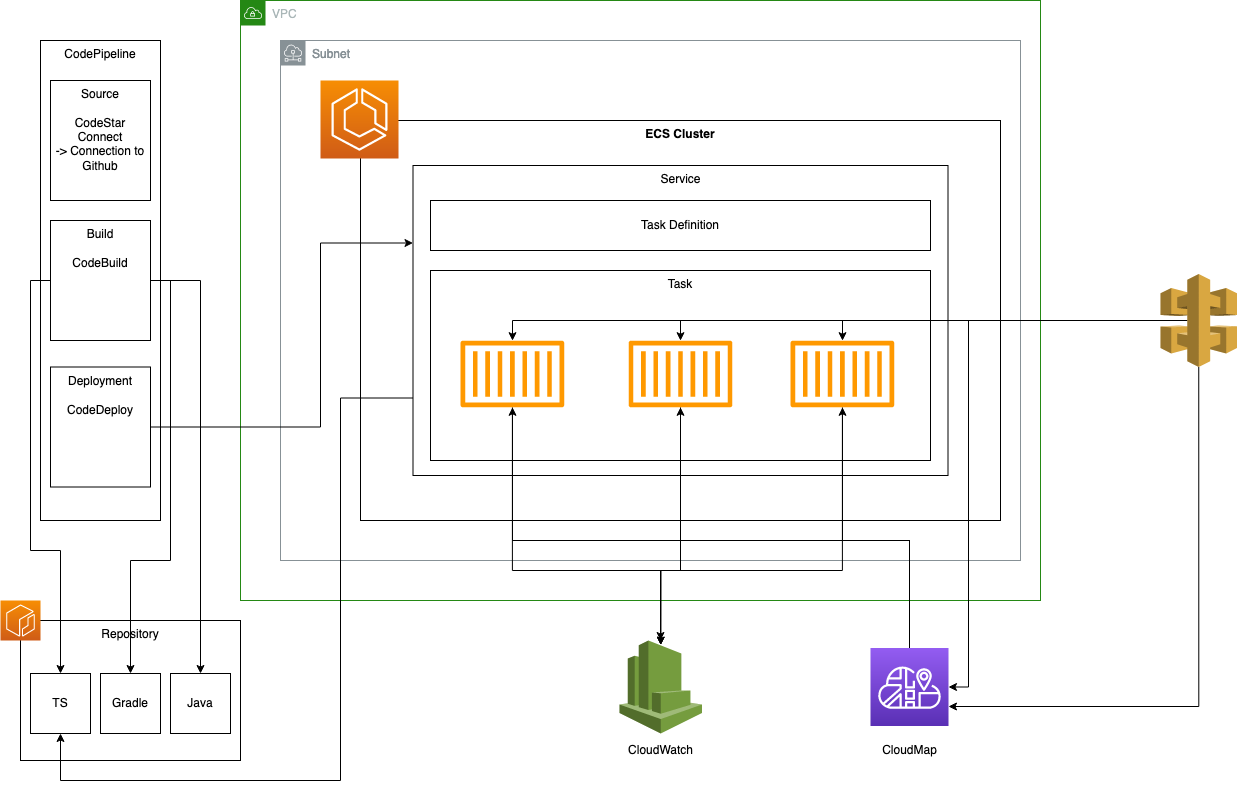
\includegraphics[width=\textwidth]{aws_architecture.png}
    \caption{Architekturentwurf für die AWS-Services}
    \label{fig:CloudArchitektur}
\end{figure}

Ziel ist es, die Anwendung auf Containern zu deployen. Dazu wird \ac{ECS} zur Bereitstellung eines Clusters mit Containern. Innerhalb des Clusters ist in einer \textit{Taskdefinition} festgelegt, wie die Container laufen und unter anderem auch viele Container gestartet werden sollen und die \textit{Task} selbst, in welcher die Container bereitgestellt werden. Die Wahl ist deshalb auf \ac{ECS} gefallen, weil hier mit \gls{Fargate}, wie bereits im vorhergehenden Kapitel erwähnt, das serverless Deployment von Containern ermöglicht wird und \ac{ECS} die nicht-funktionalen Anforderungen der Skalierbarkeit und Fehlertoleranz bietet. \pagebreak

Das \ac{ECS} Cluster selbst befindet sich innerhalb eines von einer \ac{VPC} bereitgestellten Subnetz. Erreichbar sind die einzelnen Container über ein \textit{API Gateway}, ein zentraler API Endpunkt, welcher auf die IP-Adressen innerhalb des Subnetzes verweist und das Load-Balancing zwischen den einzelnen Instanzen übernimmt. Die Adressen der Container werden in \textit{CloudMap} als Service Registry gespeichert und der Betrieb der Container mit \textit{CloudWatch} überwacht. \textit{CloudWatch} orchestriert die Logs der einzelnen Container zentral für optimales Monitoring.

Neben dem \ac{ECS} Cluster wird als weiterer Service \textit{\gls{CodePipeline}} eingesetzt, welcher eine \ac{CI/CD}-Pipeline bereitstellt. \ac{CI/CD} bedeutet, dass neue Anwendungsversionen automatisiert deployed werden, wenn eine Aktualisierung im Anwendungscode implementiert wird. 

\textit{\gls{CodePipeline}} Kombiniert die Services \textit{CodeStar}, \textit{CodeBuild} und \textit{CodeDeploy}. \textit{CodeStar} stellt hierbei eine Verbindung zu \gls{GitHub} her, wo der Anwendungscode abgelegt ist. \textit{CodeBuild} erzeugt ein Abbild der Anwendung in einem Container und legt diesen in \ac{ECR} ab. \textit{CodeDeploy} deployed die aktuellste Version der Anwendung über \ac{ECS} in das Cluster.

Das Bereitstellungsmodell entspricht letztendlich dem \ac{CaaS} Modell, also der Bereitstellung von Containern, ohne der Notwendigkeit die zugrundeliegende Hardwareplattform zu konfigurieren, da diese Aufgabe von \gls{Fargate} übernommen wird.

Definiert wird die Infrastruktur zuvor in einem \gls{Terraform} Skript, in welchem beschrieben wird, welche Services bereitgestellt werden und wie diese untereinander kommunizieren.